\documentclass{report}
\usepackage{pdfpages}
%\usepackage[cyr]{aeguill}
\usepackage[utf8]{inputenc}
\usepackage{xspace}
\usepackage[francais]{babel}
\usepackage{listingsutf8}
\usepackage{graphics}
\DeclareUnicodeCharacter{B0}{\textdegree}
\renewcommand{\contentsname}{Sommaire}
\usepackage[T1]{fontenc}

\date{\today}
\author{}
\title{}
\makeatother
\title{Rapport de projet tutoré : Développement d'un System-On-Chip open-source}
\author{\bsc{DUZAN} Luc \and \bsc{LONGO} Matthieu \and \bsc{FARACHE} Gabriel \and \bsc{MICHAUD} Clément }

\date{20 janvier 2012}

\begin{document}

\maketitle

\tableofcontents

\chapter*{Introduction}
    Les systèmes électroniques numériques sont constitués de bascules (permettant de
sauvegarder des états logiques) et de portes logiques (et, ou, non, ou exclusif par
exemple) interconnectés entre elles. Ces portes sont elles-mêmes constituées de
transistors qui sont donc les briques élémentaires de l'électronique numérique. En
effet, elles peuvent être utilisées comme de minuscules interrupteurs pilotés. Il est
possible de graver un enchevêtrement complexe de transistors sur une seule plaque de
silicium, on parle de circuit intégré.  Concevoir un circuit intégré consiste alors à
choisir des portes logiques et des bascules et à définir des connexions entre elles
afin d'obtenir le comportement désiré.  Les portes logiques sont aussi décrites par
des réseaux de transistors.  Au final, un circuit intégré est construit en gravant un
complexe réseau de transistors sur une seule plaque de silicium.

Historiquement ce réseau complexe était dessiné à la main sur des feuilles spéciales
(feuilles de mylar) ce qui limitait fortement la complexité des circuits intégrés. De
plus, il n'était pas possible de tester la conception sans la graver. La montée en
puissance des ordinateurs a alors permis la mise en place de langages de description
de matériel (appelés HDL pour \textit{hardware description language}). Les HDL
permettent de modéliser le comportement des circuits logiques et également de décrire
les structures de ces circuits logiques, on peut alors simuler le comportement de la
structure décrite et vérifier qu'elle se comporte de manière conforme au modèle. Il
est souvent possible de déduire de manière automatique la description structurelle
d'un circuit à l'aide de sa description comportementale. L'apparition de ses langages
a alors révolutionné le monde de la conception des circuits intégrés. Les concepteurs
décrivent alors leurs circuits grâce aux HDL, les simulent de manière virtuelle et
génèrent automatiquement à l'aide de synthétiseurs les dessins physiques qui
représentent le circuit intégré, ces dessins appelés netlists sont ensuite envoyés à
une fonderie qui s'occupe alors de la fabrication. Une fonderie est une entreprise
spécialisée dans la fabrication de circuits. Ces nouvelles techniques de production
permettent alors de produire des circuits intégrés spécifiques à des attentes
particulières plutôt que d'utiliser des microcontrôleurs et de les programmer afin
d'obtenir le comportement attendu, il s'agit d'ASIC pour \textit{Application Specific
Integrated Circuit}. Cependant la conception et surtout la fabrication d'ASIC ne
peuvent être rentabilisées que pour de gros volumes de production, de plus une erreur
de conception sur un ASIC peut coûter très chère. Mais l'apparition des FPGA (pour
\textit{Field Programmable Gate Array}), qui sont des circuits intégrés logiques
reprogrammables après leur conception, marque encore une fois une révolution.  Ils
permettent de tester de manière plus poussée la conception d'ASIC en créant des
prototypes et peuvent même être vendus une fois programmés à la place d'ASIC pour des
petits volumes de production. Les FPGA de nos jours sont assez performants pour
contenir l'intégralité des composants nécessaires au fonctionnement d'un système
complet (microprocesseur, mémoire, GPIO, ...), on parle alors de SoC. Les SoC
(\textit{Systen On Chip}) désignent un système complet qui est contenu sur une seule
puce que ce soit un FPGA ou un ASIC.

Dans notre projet tutoré, nous allons nous intéresser plus particulièrement au
\textit{Milkymist} SoC, qui est un SoC \textit{open-source}, c'est à dire que le code HDL qui le décrit
est libre de droit.  Ce SoC a été conçu pour être programmé sur un FPGA spécifique le
Virtex-4 XC4VLX25.  Notre but est d'adapter le code de ce SoC pour le rendre
compatible avec le Xilinx Spartan6 qui est utilisé à l'INSA de Toulouse.  Nous
allons aussi ajouter un module à \textit{Milkymist} permettant d'exploiter la propriété de
certains FPGA qui est de pouvoir être reprogrammé à la volée. C'est-à-dire que nous
allons permettre au système \textit{Milkymist} de pouvoir ajouter à chaud (sans redémarrer le
système) des périphériques (à partir de leurs descriptions structurelles) sur le FPGA
et de les connecter au SoC.

Ce rapport ayant pour but de clarifier le travail de notre projet tutoré, nous allons
dans un premier temps détailler la conception des circuits intégrés.  Pour cela, nous parlerons
dans un premier temps des supports pouvant recevoir des circuits intégrés (FPGA et ASIC),
nous parlerons ensuite de la conception du matériel à l'aide des langages de
description de matériel tel que VHDL, Verilog et Migen et nous ferons un état sur
l'avancement de la communauté \textit{open-source} dans ce domaine.  Dans la deuxième partie,
nous parlerons ensuite du projet \textit{Milkymist} et de l'intention de notre contribution
sur ce projet.


\chapter{Conception du matériel}

\section{Technologie de conception}
    \subsection{ASIC}

\subsubsection{Netlist} Une fois la conception réalisée à l'aide de langages de
descriptions matériel, on peux obtenir une netlist du circuits intégrés. Cette
netlist contient dans un premier temps, une liste qui défini les composants utilisés
dans ce circuit intégré, chaque composant est définie par les différents points de
connexion (appelé \textit{port}) qu'il possède et par ses propriétés élémentaires. Un
composant peut être quelque chose d'élémentaire comme un transistor ou une résistance
tout comme un complexe circuit intégré. Ensuite la netlist va alors décrire des
connexions entre des composants. Chaque composant décrit dans le réseau est forcement
un des composants de la liste précédemment décrite, on dit alors que ce composant est
une instance de la définition donnée dans la liste de composants. Les connexions sont
décrites par une liste de fils. Un fil connecte un port donné d'une instance avec un
autre port donné d'une autre instance. Pour limiter la redondance, on peut
hiérarchiser les netlists, c'est à dire que l'on peut ranger une partie d'une réseau
dans une définition d'un composant. De cette manière si cette partie est répétée
plusieurs fois dans le réseau, on peux l'insérer comme on insérerait un composant
élémentaire, et la description de cette partie est alors donnée qu'une seule fois.

\subsubsection{Fabrication d'ASIC}

\begin{figure}
\begin{center}
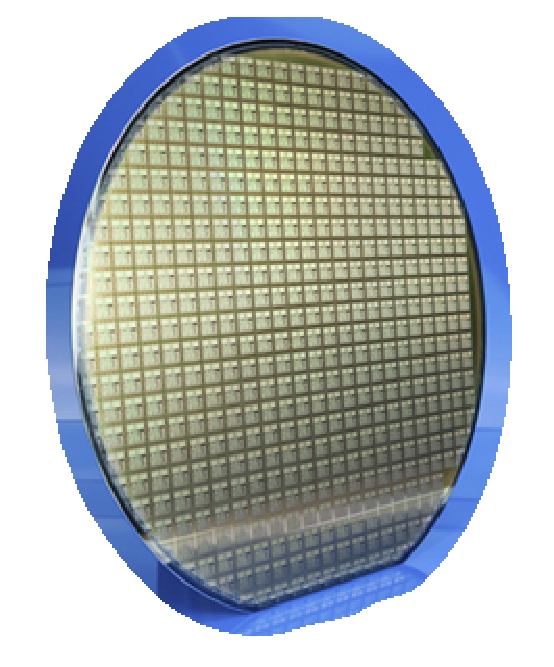
\includegraphics[scale=0.4]{asic.eps}
\end{center}
\end{figure}

A partir de la description en netlist, il est possible d'obtenir un fichier
(généralement au format GDSII) qui représente le dessin physique du circuit intégré.
C'est à dire qu'il représente entre autre les formes géométriques à graver sur le
silicium, c'est ce fichier qui est envoyé aux fondeurs. Ce fichier permet alors
d'obtenir les masques nécessaires à la gravure du système. Ce procédé utilisant le
plus souvent la lithographie est très complexe et ne sera pas détaillé dans ce
rapport. La fabrication d'ASIC demande un fort investissement en matériels, c'est
pour cela qu'on observe une séparation entre les entreprises qui conçoivent les
circuits intégrés et les fonderies car il faut une très grande production pour
amortir les investissements. Seul quelques entreprises tel que Intel,
STMicroelectronics, Texas Instruments qui produisent de très grands volumes peuvent
se permettre de faire en même temps la conception et la réalisation de leurs
circuits. Les ASIC ne peuvent alors être réalisé pour un prix raisonnable en petit
volume.


\subsection{FPGA}

\begin{figure}
\begin{center}
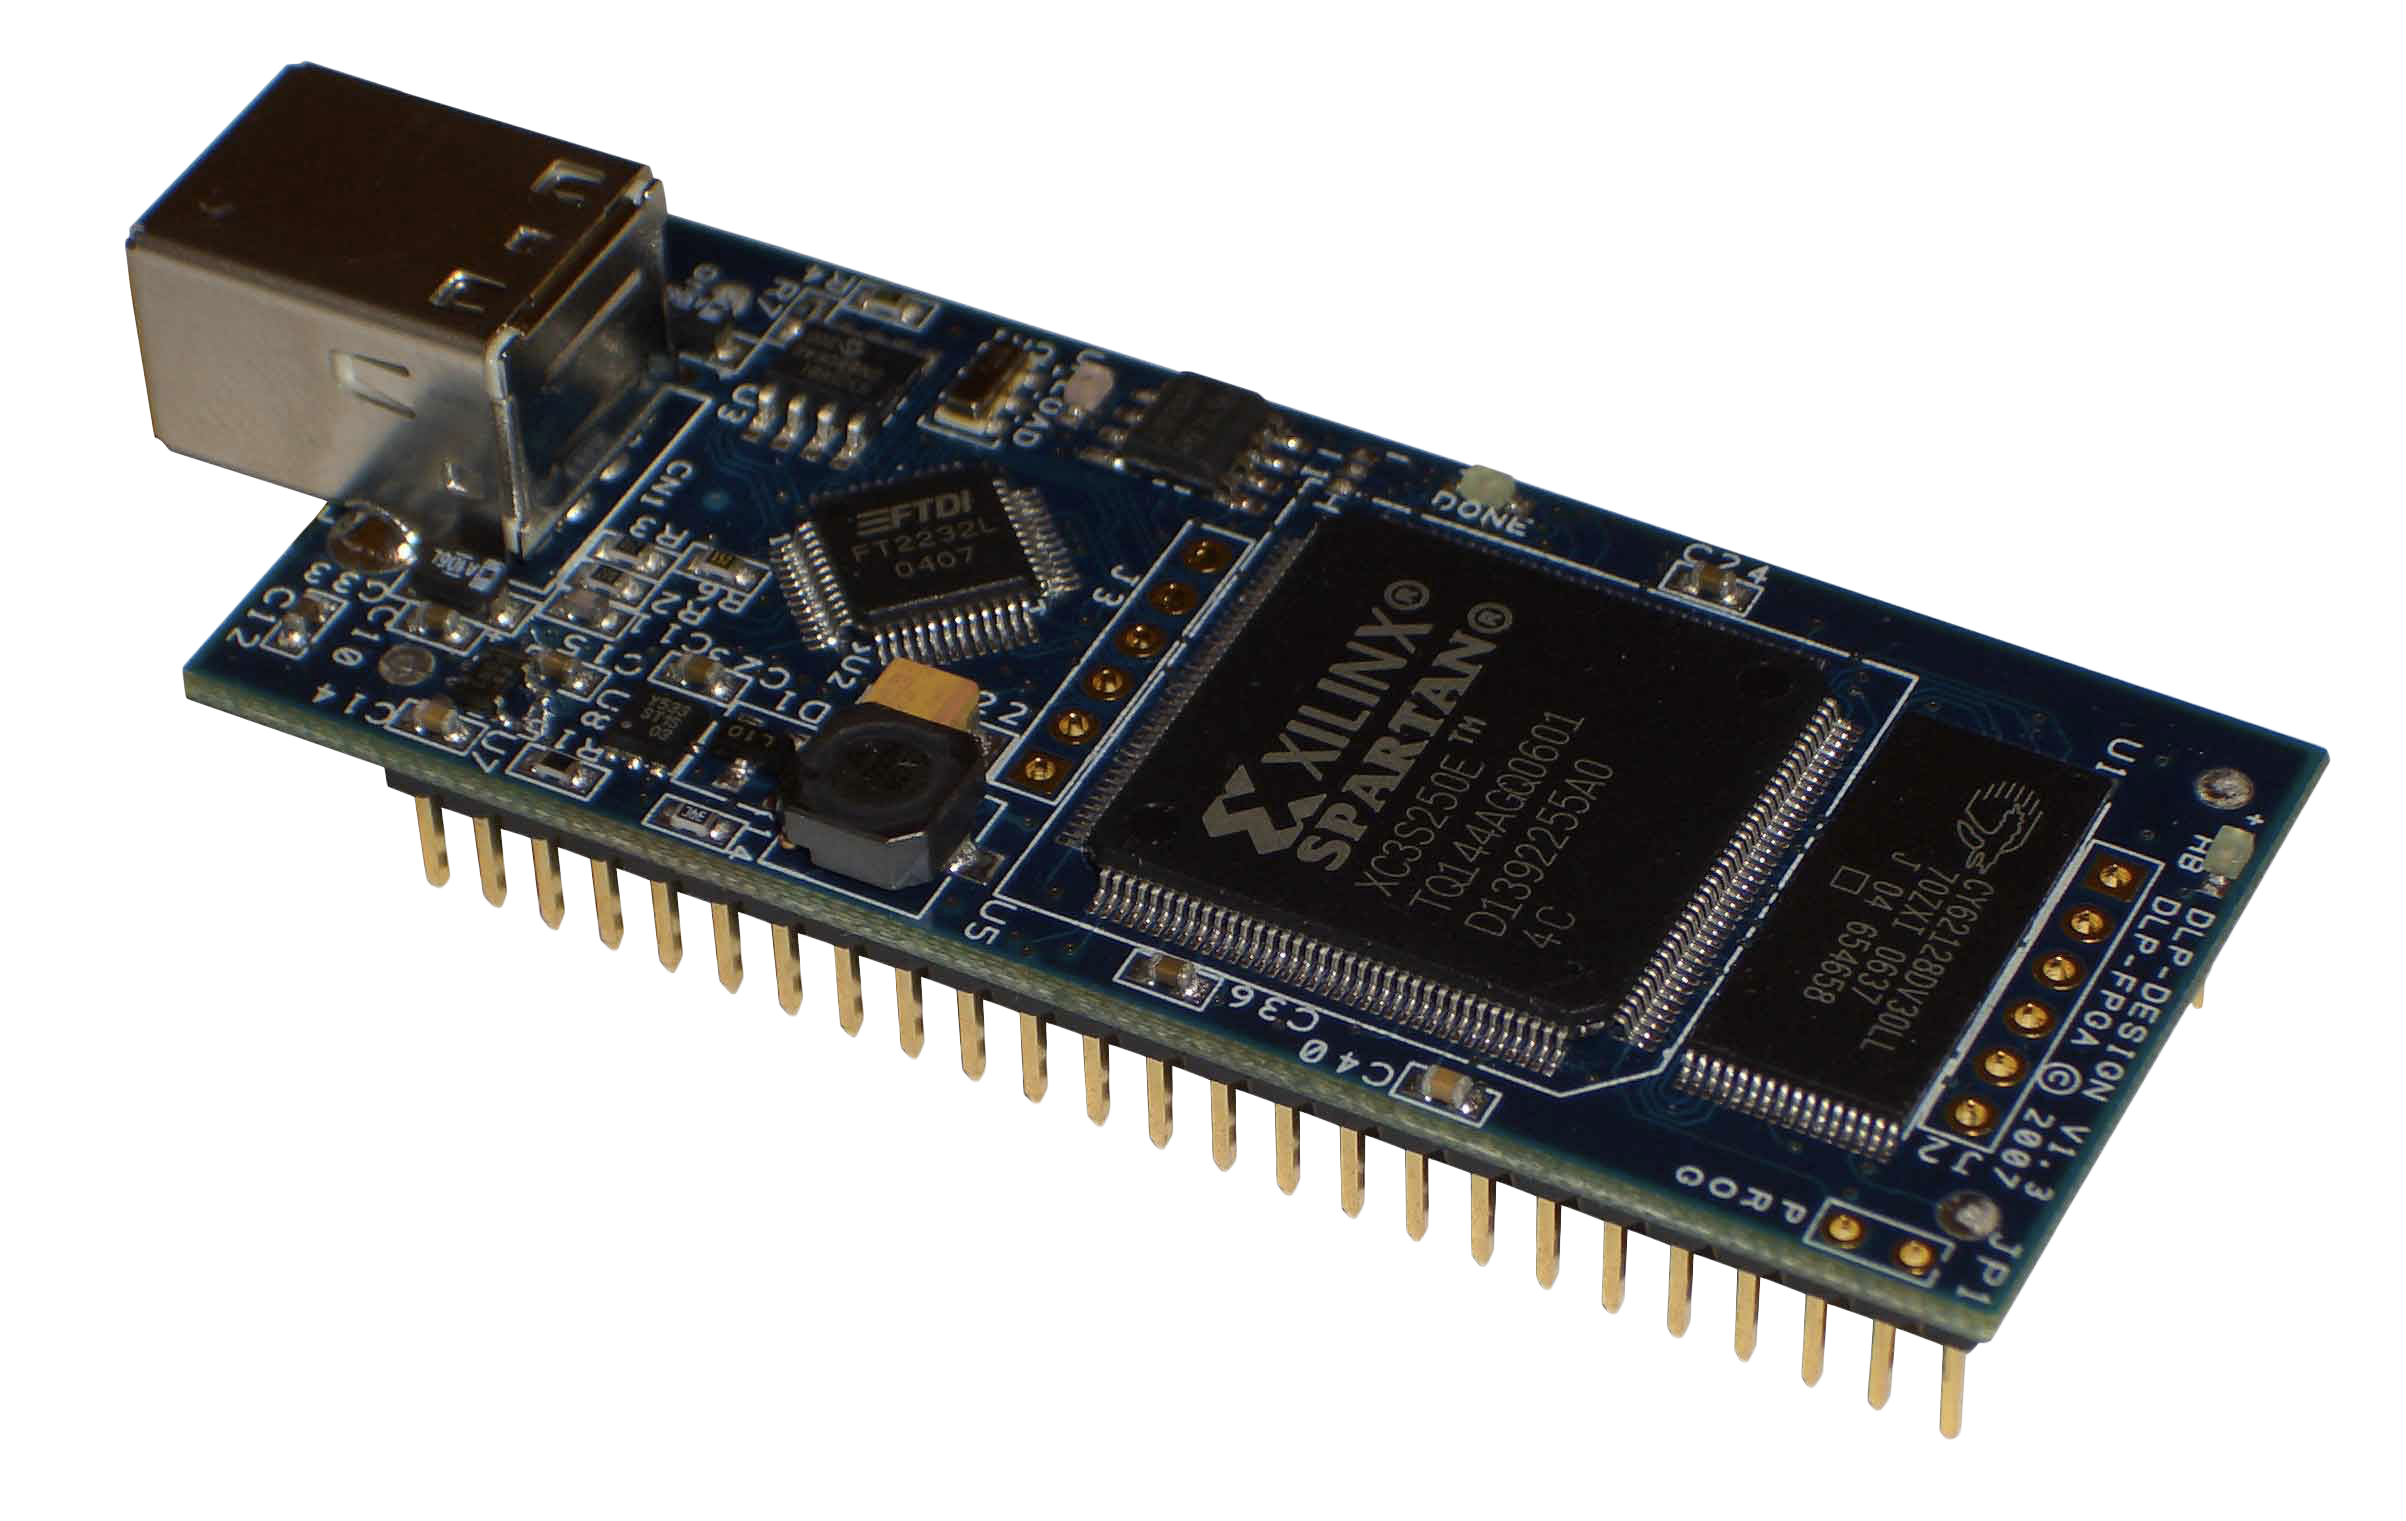
\includegraphics[scale=0.1]{fpga.eps}
\end{center}
\end{figure}

Les FPGA (\textit{Field Programmable Gate Array}) sont des circuits logiques
programmable. En effet \textit{Field Programmage} signifie programmable sur le champ,
le circuit peut être programmé après sa fabrication pour réaliser n'importe qu'elle
fonctions logiques. La configuration d'un FPGA est obtenu à l'aide de langages HDL
qui permettent aussi de concevoir les ASIC, c'est pour cela que les FPGA peuvent être
utilisés pour faire des prototypes d'ASIC.

Les FPGA sont constitué d'un nombre très importants de bloques logiques rangés en
matrice (d'où le \textit{Gate Array} de FPGA). C'est bloques logiques peuvent être
configurés pour effectué des fonctions logiques élémentaires (et, ou, ou exclusif,
non) ou quelques fonctions logiques plus complexes. Ils peuvent aussi être configurer
en bascule ou en d'autres éléments permettant de mémoriser de l'information. Ces
bloques logiques peuvent également être connectés de manière arbitraire entre eux.
C'est en définissant les fonctions réalisées par ces bloques logiques et des
connexions entre eux que l'on peut configurer un FPGA pour obtenir le fonctionnement
attendu. Cette configuration est générée de manière automatique à partir de
description en HDL. De nos jours le nombre de bloques logiques sur les FPGA se compte
en millions. 

Les cartes FPGA contiennent en plus du réseau de bloques logiques programmable des
périphériques. Cela permet d'économiser des portes, de plus certains périphériques
tel que les GPIO ne peuvent pas être programmés à l'aide de bloques logiques. Il
n'est donc pas rare de voir des cartes FPGA embarquait des GPIO, de la RAM, des
cartes réseaux par exemple. Dans notre projet tuteuré, la différence des
périphériques utilisés par la carte FPGA utilisé à l'INSA et celle utilisé par
MilkyMist entrainent des problèmes de portabilités.

\begin{center}
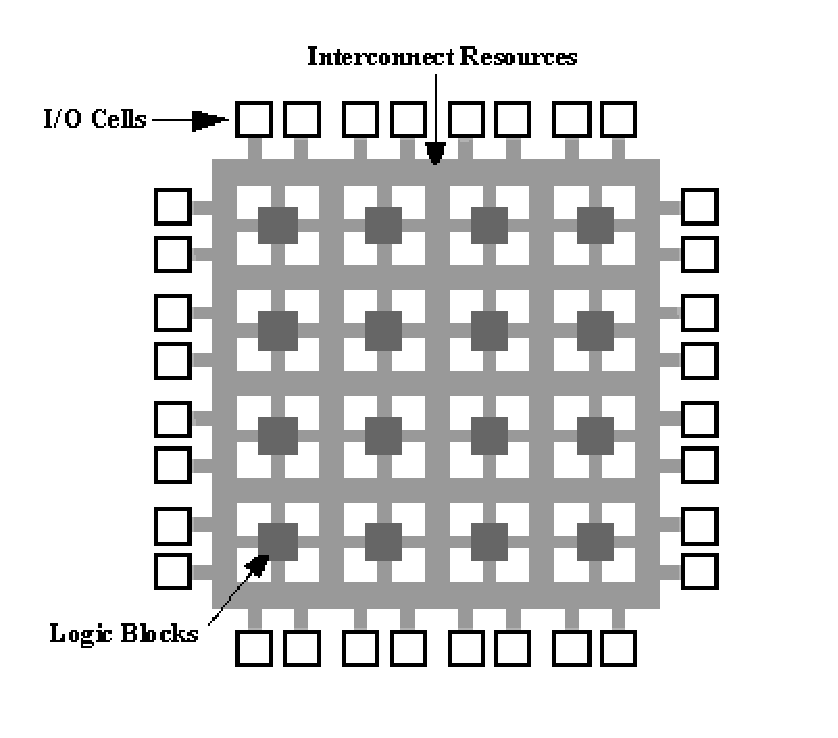
\includegraphics[scale=0.5]{porte.eps}
\end{center}

    \newpage

\section{Langage de description de circuit logique}
    \vspace{15px}
\subsection{Présentation de Verilog et VHDL}
\vspace{15px}
Verilog et Very high speed integrated circuit Hardware Description Language ou VHDL sont tous deux des Hardware Description Language ou HDL soit en français Langage de Description de Matériel. Les HDL utilisent une méthode de description de flux de processus résultant d'un modèle de flux de données avec des informations de synchronisation (le temps). Cette méthode consiste en une abstraction au niveau des portes logiques et des transitors. Cette méthode s'appelle Register-Transfer Level ou RTL et a été défini à cause de l'explosion de la complexité des circuits électroniques depuis les années 1970 (loi de Moore). En effet, les concepteurs de matériel micro-électronique avaient besoin d'une méthode de description logique des matériel numériques de plus haut niveau pour limiter la complexité de la conception et cela sans que cette dernière ne soit spécifique à une technologie en particulier. Les HDL utilisent donc cette méthode pour représenter des circuits à un niveau élevé. A partir de cette représentation des circuits, des représentations de plus bas niveaux et le cablage peuvent être déduit. Les HDL permettent donc de décrire un circuit électronique tant au niveau comportemental que structurel, c'est-à-dire les flux de signaux transitant entre les différents registres. C'est pour cette simplification dans la conception et l'utilisation des matériels que les HDL sont largement utilisés dans l'industrie.
\newpage

\begin{figure}
\begin{center}
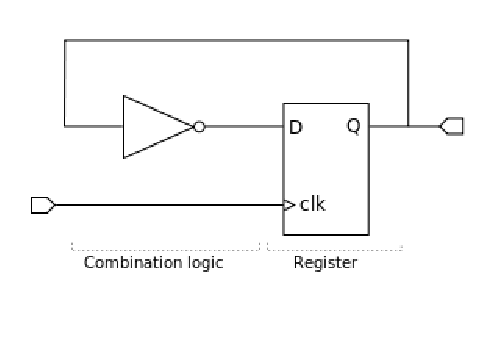
\includegraphics[scale=0.8]{rtl_example.eps}
\end{center}
\caption{Légende}
\label{Référence}
\end{figure}

Le schéma ci-dessus montre comment est représenté un circuit. Nous constatons qu'il est ici totalement fait abstraction des comment ce dernier est câblé. Nous ne connaissons que ce qui entre et ce qui sort de ce dernier. Un HDL décrira quant à lui le "comportement" externe, générale du circuit.

La principale différence entre les HDL avec les langages de programmations traditionnels est qu'avec un HDL, contrairement aux autres type de langage procédurier, nous pouvons modéliser de multiples processus parallèles et exprimer le temps de manière explicite. En effet, ces deux éléments (le parallélisme et le temps) sont les principaux attributs d'un matériel électronique. Un changement dans un des processus pourra donc déclencher une mise à jour dans les autres processus.

\subsection{Les autres HDL existant}
\vspace{15px}
Il existe de nombreux HDL autre que les deux plus connu que sont Verilog et VHDL, tel que, Altera HDL (AHDL) qui est un langage propriétaire d'\textbf{Altera}, Hydra qui est basé sur \textbf{Haskell}, MyHDL qui est basé sur \textbf{Python} ou encore RHDL basé sur \textbf{Ruby}. Un autre HDL est SystemC, qui est, avec Verilog et VHDL, un des HDL les plus utilisés dans l'industrie. Cependant, ce dernier n'est pas un langage à part entière puisque c'est en fait un ensemble de classes \textbf{C++} fournissant les outils nécessaires à la modélisation du matériel. De part cette caractéristique, nous ne nous y attarderons pas plus. Milkymist, ceux qui font le SoC sur lequel nous allons travailler, possède aussi leur propre langage Migen qui est toujours en développement, nous y reviendrons plus loin dans cette partie.

\subsection{Verilog VS VHDL}
\vspace{15px}
Nous allons vous présenter plus en détail les deux principaux HDL que sont VHDL et Verilog. Chacun à ses atouts :
\begin{itemize}
\item VHDL :
\begin{itemize}
\item ce langage a été fait pour aider la conception et la spécification au niveau d'un système électronique,
\item il est plus souple que Verilog car permet, entre autre, à l'utilisateur de définir ses types, ses configurations, etc.
\end{itemize}
\item Verilog :
\begin{itemize}
\item conçut de base pour les concepteurs de matériel numérique développant des FPGAs et ASICs
\item parfait pour convertir des types de données de vecteurs de bits vers des notations arithmétiques,
\item existence de supports compréhensible pour la conception numérique de bas niveau.
\end{itemize}
\end{itemize}

Ce sont-là les principales différences entre les deux langages. Dans les fait, VHDL et Verilog sont similaires puisqu'ils sont tous les deux des standards IEEE : \textit{IEEE standard 1076} en 1987 puis \textit{IEEE standard 1076-1993} en 1993 après une mise à jour pour VHDL. Il a ensuite été mis à jour régulièrement pour arriver, en 2008 au standard \textit{IEEE 1076-2008} (VHDL 4.0) qui est la dernière version en date. Verilog est lui devenu un standard en 1995 : \textit{IEEE standard 1364-1995} et a été mis à jour deux fois depuis : en 2001  \textit{IEEE Standard 1364-2001} (Verilog 2001) qui corrigera de nombreux problèmes puis en 2005  \textit{IEEE Standard 1364-2005} (Verilog 2005) qui corrigea quelques bugs.. Historiquement, VHDL a été développé pour l'armée de l'air des Etats-Unis d'Amérique (contrat \textit{F33615-83-C-1003}) par \textit{Intermetrics, Inc.}, \textit{Texas Instruments} et \textit{IBM}. \textit{Intermetrics, Inc.}  fournissait les experts en langage (de programmation) et était aussi le maître d'\oe{}uvre du projet. \textit{Texas Instruments} se concentrait sur la partie expertise en conception de puces (électronique). \textit{IBM} quant à lui fournissait les experts en conception de systèmes informatiques. C'était donc un projet d'une certaine envergure (comme \textit{ADA} par exemple). Verilog a quant à lui était lancé en 1984 par \textbf{Gateway Design Automation Inc.}  puis rendu disponible au grand public en 1990 par \textbf{Cadence}.

\subsection{Le HDL de Milkymist : Migen}
\vspace{15px}
Nous vous avions aussi parlé de Migen, le langage de Milkymist. Nous n'allons pas l'uitliser mais il nous semblait intéressant d'en parler. En effet, dans le futur, le SoC Mylkymist utilisera ce langage. Le projet Migen (pour \textbf{Mi}lkymist \textbf{gen}erator) a été lancé en 2011 et est toujours en cours de de développement. Cet outil est basé sur le langage python et il a pour but d'automatiser encore plus le processus de conception des VSLI (Very-large-scale integration, c'est un processus de création de circuits intégrés). Grâce à Migen, il sera possible d'appliquer des concepts modernes, tel que l'objet et la métaprogramation par exemple, pour concevoir un matériel. L'avantage étant que ce qui en résulte est plus élégant et est surtout plus facile à faire évoluer, tout en réduisant les problèmes dûs aux erreurs humaines. Ce sont-là les grands principes que Milkymist veut mettre en place dans Migen. En se basant sur ces dernières, Migen fournira les outils nécessaires pour construire des conceptions synchrones de manière plus productive en automatisant certaines tâches comme réinitialiser les registres et en faisant abstraction du paradigm des HDL basé sur l'évènement (le parallélisme). Migen permettra aussi d'intégrer le Soc (system-on-chips) en automatisant par exemple l'interconnexion entre les chips (puces). Migen accélérera aussi la conception matériel grâce le paradigm du flux de données avec une intégration semi automatique dans le Soc.

Migen semble donc un projet très intéressant puisqu'il rend la conception plus simple et qu'il rend plus efficace le matériel. Cependant, ce projet est encore jeune et encore en développement, toutes les fonctionnalités ne sont pas encore implémentées. Nous ne l'utiliserons donc pas dans notre projet pour éviter tout problème.

    \newpage

\section{Le monde de l'open source et son avancement sur les FPGA}
    \vspace{15px}
\begin{minipage}{0.40\linewidth}
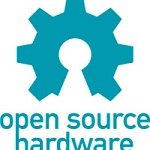
\includegraphics{oshw-logo.jpg}
\end{minipage}\hfill
\begin{minipage}{0.55\linewidth}
Dans cette partie nous allons parler des matériels open-source, c'est à dire que les matériels, ou plutôt leurs conceptions, sont crées de manière communautaire ou par des sociétés privée. Ils ne sont pas soumis à des brevets ultra-restricitfs mais qui sont le plus souvent sous licence GPL (General Public License) ou assimilé plus souples. 
\end{minipage}
\medskip
Le materiel open-source est très peu developpé contrairement à son homologue loigiciel. Il n'y a que peu d'acteurs sur cette scène alors qu'il y en a des dizaines pour l'open-source logiciel. Cependant, ce pan de l'open-source tend de plus en plus à se developper ces derniers temps. Pour preuve, en 2010 a été publié le \textbf{Open Source Hardware} (\textbf{OSHW}). Il s'agit d'une définition de ce qu'est un matériel open-source et des idéaux de ce dernier..
\medskip
Il y a d'autres projets en cours, que ce soit dans le domaine des ordinateurs eux-mêmes, dans leur composants (CPU (\textit{Central Processing Unit}, le coeur de la machine), carte graphique, ...), voir même dans d'autres secteurs tels que la téléphonie et le GPS. Voici la liste des projets open-source relatifs aux ordinateurs : \textit{Arduino}, \textit{Beagle Board}, \textit{Bug Labs}, \textit{CuBox}, \textit{Ethernut}, \textit{GP32}, \textit{Maple}, \textit{PLAICE}, \textit{Raspberry Pi}, \textit{Simputer}, \textit{Pandora}, \textit{PC532} qui date des années 1990, \textit{Minimig} qui est une nouvelle implémentation de l'Amiga 500 utilisant des FPGA, \textit{Milkymist One} qui est un carte-ordinateur implémentant tous les principes logiques à travers des fichiers de conception créés avec \textit{Verilog}. Ces fichiers sont open-source, donc disponible à tout le monde. Dans la plupart des autres matériel open-source, ces fichiers sont confidentiels et propriétaire. Bien évidemment, cette carte utilise \textit{Milkymist SoC} comme CPU.
\medskip
En parlant de CPU, nous pouvons aussi lister les différents projets : \textit{Amber}, \textit{LEON}, \textit{OpenCores}, \textit{OpenSPARC}, \textit{OpenRISC} qui est plus un groupe de développeur visant à créer des CPU RISK ayant des performances très importantes. Enfin, le \textit{Milkymist SoC}, coupellé au micro-processeur \textit{LatticeMico32}, qui possède un ensemble de SoC développé de manières indépendant et open-source. Nous constatons qu'il y a bien moins de projet open-source concernant les CPU que les ordinateurs eux-mêmes.
\medskip
La plus grosse communauter à l'heure actuelle est OpenCores (\URL{www.opencores.org}). Fondée en 1999 par Damjan Lampret, OpenCores (OC) a commendé a developpé \textit{OpenRISC 1000}. Le développent s'est poursuivi jusqu'en 2007. Durant cette période OC a été supporté par \textit{Flextronics}. A partir de 2007, \textit{OpenRISC 1000} est passé dans une phase de déploiement commerciale grâce à \textit{ORSoC AB}. En mars 2012, il y avait plus de 147 000 utitilisateurs enregistrés et plus de 900 projets en cours sur cette architecure matériel. \textit{ORPSoC} est l'implémentation de SoC de référence sur cette architecture. Cepedant, le \textit{Raspberry Pi} (raspi), l'ordinateur à 29\$ sortie courant 2012 grossit de plus en plus. De nombreuses cartes electroniques complémentaire au raspi sont sortient, toutes dans un prix raisonable. Un projet de sortir une caméra est même en cours et son prix devrait lui aussi être extremement raisonable compte tenu de la technologie impliqué. 
\medskip
Il faut savoir que contrairement aux idées reçus, les entreprises qui font de l'open-source hardware ont de (très) bons résultats. En effet, les 13 plus grosses sociétés qui ont ce genre d'activités ont toutes plus d'un million de dollars de chiffre d'affaire (en dollars et en 2010) :
\begin{itemize}
\item Adafruit Industries : plus d'1 million
\item Arduino : plus d'1 million
\item BeagleBoard : 1 million
\item Bug Labs : 1 million
\item Chumby : plus d'1 million
\item Dangerous Prototypes
\item DIY Drones : 1 million
\item Evil Mad Scientist  Labs
\item Liquidware : plus d'1 million
\item MakerBot Industries : 1 million
\item Maker Shed : plus d'1 million
\item Parallax : plus d'1 million
\item Seeed Studios : 1 million
\item Solarbotics : plus d'1 million
\item SparkFun Electronics : 10 millions
\end{itemize} 
Ces entreprises ne sont qu'un échantillon, il existe bien d'autres entreprises de ce type qui dépassent ou approche le million de chiffre d'affaire. De plus ces chiffres datent de 2010, on peut donc légitimement supposé que ces chiffres ont évolués de manières positives ces deux dernières années. De plus, selon les prévisions, en 2015, le chiffre d'affaire cumulé de toutes les entreprises de matériel open-source devrait avoisiné le milliard de dollars.
\medskip
Ce secteur a donc un avenir radieux qui s'offre à lui, de plus en plus de projet voient le jour et ceux qui sont déjà présents ne font que s'améliorer grâce au travail que donne toutes les personnes possédant ce genre de matériel, car c'est bien là le leitmotiv de l'open-source : la progression par la participation.

    \newpage

\chapter{Adaptation d'un System On Chip libre : MilkyMist}
\newpage

\section{Le projet MilkyMist}
    Ce projet a pour origine le projet de fin d'étude de Sébastien Bourdeauducq \cite{BOURDEAUDUCQ} sur le design d'un System-on-Chip au Royal Institute of Technology de Stockholm en 2010. Plus précisément, il s'agissait de réaliser un SoC rapide et économe en ressources, basé sur FPGA et avec pour but principal de supporter une application de rendu d'effets video en temps réel. Ces effets peuvent être aussi bien réalisés avec un ordinateur normal. Cependant cette approche a certains inconvénients, un système embarqué a l'avantage d'être moins encombrant et plus facile à mettre en place. Le temps de démarrage et de configuration est réduit à  quelques secondes contairament à un ordinateur normal qui doit d'abord lancer un système d'exploitation lourd tel que Windows et ensuite lancer un logiciel spécialisé permettant de créer des effets vidéo. De plus, on peut avoir des interfaces spécialisées qu'un PC normal n'a pas, à moins de les rajouter, ce qui peut se révéler assez cher.


Le SoC \textit{Milkymist} est implémenté sur un FPGA et utilise le coeur LatticeMico32 (LM32)\cite{LATTICE}. C'est un CPU 32-bit \textit{big endian} RISC \textit{open-source}. Le microprocesseur LM32 est assisté dans son travail par une unité de mappage de texture et par un coprocesseur programmable à virgule flottante qui est utilisé par le logiciel de synthèse video.
    \newpage

\section{Le travail à réaliser}

\subsection{Portage sur le Nexys3}
    \vspace{15px}

Un SoC est composé de blocs correspondant chacun à un module spécifique (CPU, interfaces RS232, USB, PCI, modules de traitement du signal, blocs réseaux ARM ou Ethernet, module d'encryption DES ou AES ...). Heureusement il n'est pas à chaque fois nécessaire de tout réadapter. La plupart des modules écrit pour un certain projet sont réutilisables dans d'autres, ils ont été souvent prévus pour une intégration plug and play. Chacun des blocs constitue un bloc Soft-IP (Soft Intellectual Property Block) en opposition aux Hard-IP Blocks (ASIC), généralement bien documenté afin de faciliter le travail de réintégration et dont la licence encadre ses conditions de réutilisation au sein d'un projet (licence propriétaire entrainant le paiement de droit ou licences opensources avec chacune leurs partucalarités). Les avantages de blocs IP sont nombreux, ils permettent de supprimer le temps d'écriture du bloc donc diminuer le temps jusqu'à la commercialisation, diminuer le nombre d'ingénieurs requis pour le projet donc diminuation des coûts  et enfin rassurer les développeurs car la solution est déjà prouvée.\\

\begin{center}
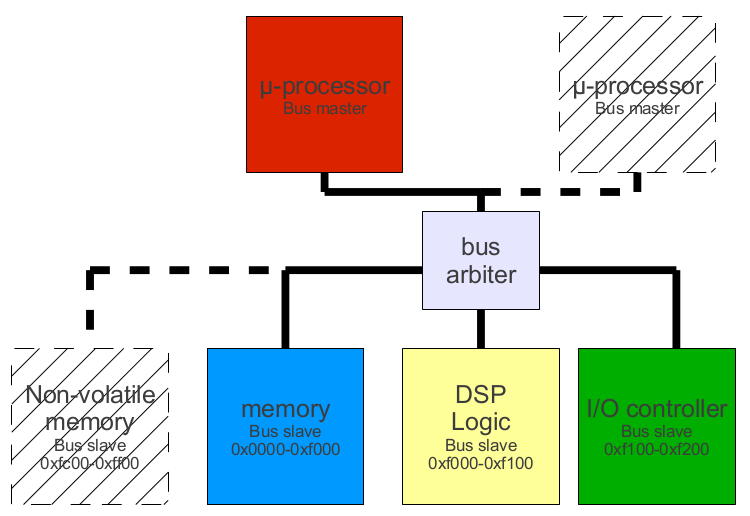
\includegraphics[scale=0.4]{soc_arch.png}
\end{center}

Seule la description du circuit (les interconnections entre les différents modules et les entrées/sorties du FPGA) est écrite à chaque fois que l'on change de carte ou/et de FPGA. Cette description peut être codée soit en VHDL ou en Verilog tout comme la description des blocs. Il s'agit souvent d'un memory-mapped bus fournissant un accès aux registres de contrôle et aux mémoires.\\

\begin{center}
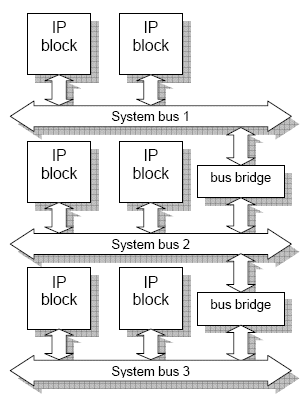
\includegraphics[scale=0.4]{soc_interconnect.png}
\end{center}

Dans notre cas, nous allons réutiliser plusieurs modules déjà implémentés. Tout d'abord, l'IP-Core LatticeMico32 (architecture RISC) déjà intégré dans MilkyMist et disponible gratuitement sous licence GNU GPL. Celui ci nécessite tout de même dû à sa généricité quelques configurations lorsqu'on le change de FPGA (taille du bus, nombre de registres, alimentation, timing, taille du cache, …) et on peut également choisir selon ses besoins d'implémenter ou non afin d'économiser des portes logiques certaines parties dans l'unité de calcul (unité de multiplication, de décalage, activer les calculs signés, ...).\\

Va être aussi réutilisé le GPIO, l'USART, la ROM qui contiendra le BIOS, … (à revoir cette partie là, y'a tellement de truc commenté et décommenté dans le fichier que c'est resté flou dans ma tête).\\

Chacun d'eux va être configuré tout comme le processeur selon nos besoins.\\

Dans cette partie, nous avons vu l'énorme utilité de la généricité dans la description des IPs. Cet espect est souvent utilisé dans l'industrie afin de créer un hardware spécifique à nos besoins. On peut gagner par cette méthode énormément en efficacité face aux architectures non-spécialisées, ce qui permet pour un résultat égal de travailler à fréquence plus basse et du coup de moins chauffer et consommer d'énergie.\\
    \newpage

\subsection{Adapter le système logiciel associé}
    Après avoir créé l'architecture qui correspond au cahier des charges du SoC,
il faut encore adapter le système d'exploitation (\textit{Operating System}) qui va le cadencer. C'est-à-dire qu'il faut récupérer un noyau existant
souvent proche de l'architecture que l'on vient de réaliser et modifier le code
pour qu'il soit entièrement compatible avec le nouveau matériel \cite{MILKY_SITE}.  Il faut tout
d'abord faire la différence entre un système d'exploitation classique que l'on
trouve sur les PC actuels permettant le traitement de tâches multiples plus ou
moins en même temps grâce au système du temps partagé (time sharing) et contenant une unité de translation des adresses physiques en adresses virtuelles
(MMU) qui gère les tâches de manière avancée et possède souvent des appels
système particuliers. En revanche les systèmes d'exploitation conçus pour les
SoC sont souvent des systèmes temps réel (\textit{Real Time OS}) qui effectuent
une tâche en continu. En effet, ceux-ci n'ont en général qu'un seul but comme
par exemple le traitement d'une vidéo dans le cas de la \textit{Milkymist One}.


Le noyau d'un système d'exploitation étant entièrement dépendant de
l'architecture du SoC, il faut généralement faire beaucoup de
modifications dans le code que l'on veut porter. C'est pourquoi il est
intéressant de sélectionner un noyau utilisé sur une architecture proche de la
nouvelle pour limiter ces modifications qui en appellent souvent beaucoup
d'autres.  Concrètement, l'un des noyaux les plus utilisés pour le SoC
est celui d'Unix. Les distributions fondées sur ce noyau et adaptés à ces
systèmes sont appelés 'linux embedded' pour embarqué. Le noyau qui se trouve à
la base de toutes les distributions unix a déjà été porté sur une multitude
d'architectures différentes comme les ARM, AVR, PIC, MIPS, SPARC, PowerPC,
etc... Une version très connue de ce linux spécial \textit{System-on-Chip} est appelé
{\bf $\mu$Clinux} \cite{UCLINUX}.  \medskip

\begin{center} 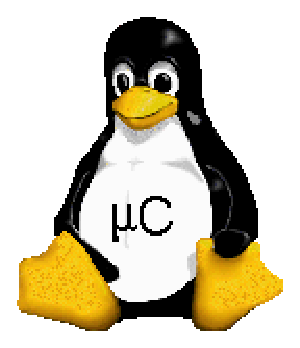
\includegraphics[scale=0.4]{uclinux.eps} \end{center}
\vspace{15px} {\Large Quelques informations sur la \textit{Milkymist}.}


Une partie de notre projet sera de porter le noyau utilisé dans la Milkymist \cite{MILKY_SITE}
pour qu'il fonctionne sur la {\bf Nexys3}. Il est important de noter que le
projet \textit{Milkymist} est l'un des premiers projets d'architecture matérielle
complètement \textit{open-source}. Le code de son gestionnaire de mémoire a d'ailleurs
été utilisé par la NASA pour construire un système totalement différent du
traitement vidéo.

La \textit{Milkymist} utilisant le processeur open source LatticeMico32 \cite{LATTICE}, il est possible
de lui associer un noyau $\mu$Clinux mais aussi un noyau {\bf RTEMS} pour
\textit{Real-Time Executive for Multiprocessor Systems}. Une multitude de drivers ont
également du être développés pour dialoguer avec les nombreux périphériques
présents sur la carte tels que les ports USB pour brancher une souris et/ou un
clavier, un port midi pour éventuellement ajouter des interactions avec un
instrument de musique, un contrôleur VGA pour afficher le résultat du
traitement, une carte son.

Une fois cette étape d'adaptation terminée nous pourrons ensuite nous lancer
dans le développement de modules propres à la fonctionnalité que nous donnerons
au système. Pour cela il suffira de développer les drivers qui accompagneront
le module. Au final, ce travail tombera dans le domaine de l'\textit{open-source} pour
que toute la communauté puisse profiter de ce portage sur la Nexys3.

Finalement ce portage ne devrait pas être très long vu que la carte possède
plus ou moins le même matériel que la \textit{Milkymist}. C'est pourquoi nous avons
décider de nous lancer dans un projet traitant un domaine en vogue : le \textit{reconfigurable computing}.


    \newpage

\subsection{Reconfiguration du materiel à la volée}
    \vspace{15px}
Le 'reconfigurable computing' est une idée qui est apparue dans les années 60 mais qui faute de capacité technologique à cette époque n'a pas pu aboutir avant 1980-90. En effet, on a commencé à graver de plus en plus de transistors sur une même surface de substrat et les chips {\bf FPGA} ont commencé à voir le jour.
L'idée majeure de ce paradigme est de joindre une partie de contrôle comprennant un processeur à une zone de logique reprogrammable à chaud. Il deviendrait alors possible de dédicacer plusieurs parties de cette logique à des tâches bien particulières qui pourraient entièrement s’exécuter en parallèle. On aurait alors un gain de cycles d'horloge considérable par rapport à un modèle classique de Von Neumann qui exécute toutes les instructions en série et décompose d'ailleurs chaque étape en fetch-decode-execute.
\medskip
Prenons un exemple simple permettant de mettre en lumière ce gain. Nous avons une machine qui possède une logique reconfigurable à chaud. Cette machine dispose également d'une carte son. Pour lire un fichier audio un système multitâche classique sera obligé de créer une tâche dédiée à la lecture de ce fichier. A différents instants, ce processus va prendre et laisser la main au processeur pour traiter les autres tâches. Le fait de valser entre les tâches et d'exécuter le processus coûte bien évidemment du temps précieux au processeur. Combien gagnerait-t-on si on créait au lieu d'une tâche, un circuit dédié qui s'occuperait indépendemment de la lecture de ce fichier et du transit jusqu'à la carte son?
\medskip
Cette tâche n'apparaîtrait plus du tout dans le planning de l'ordonnanceur et plus aucun cycle d'horloge ne serait perdu par le processeur pour exécuter cette tâche. L'idée présentée juste au dessus est à rapprocher des puces des ordinateurs classiques chargées de transiter des données d'une mémoire à une autre sans passer par le processeur (Direct Memory Access).
\medskip
Le temps gagné en n'effectuant plus ces petites tâches anodines seraient considérable. On pourrait également imaginer reconfigurer une logique qui effectue un calcul complétement dédié. On entend par là que pour effectuer un calcul complexe, on perdrait moins de temps à avoir une logique adapté à ce calcul que de passer par des cycles de décodage d'une instructions pour effectuer plusieurs calculs à la suite et obtenir enfin le résultat. Cette idée est résumée dans les 2 graphiques ci-dessous.
\medskip
On passerait d'une oprération (A+B) $>>$ C effectuer en deux temps par un modèle de Von Neumann, à un une opération exécutée en une unité de temps avec la logique reconfigurable comme illustré ci-dessous.
\medskip

\begin{center}
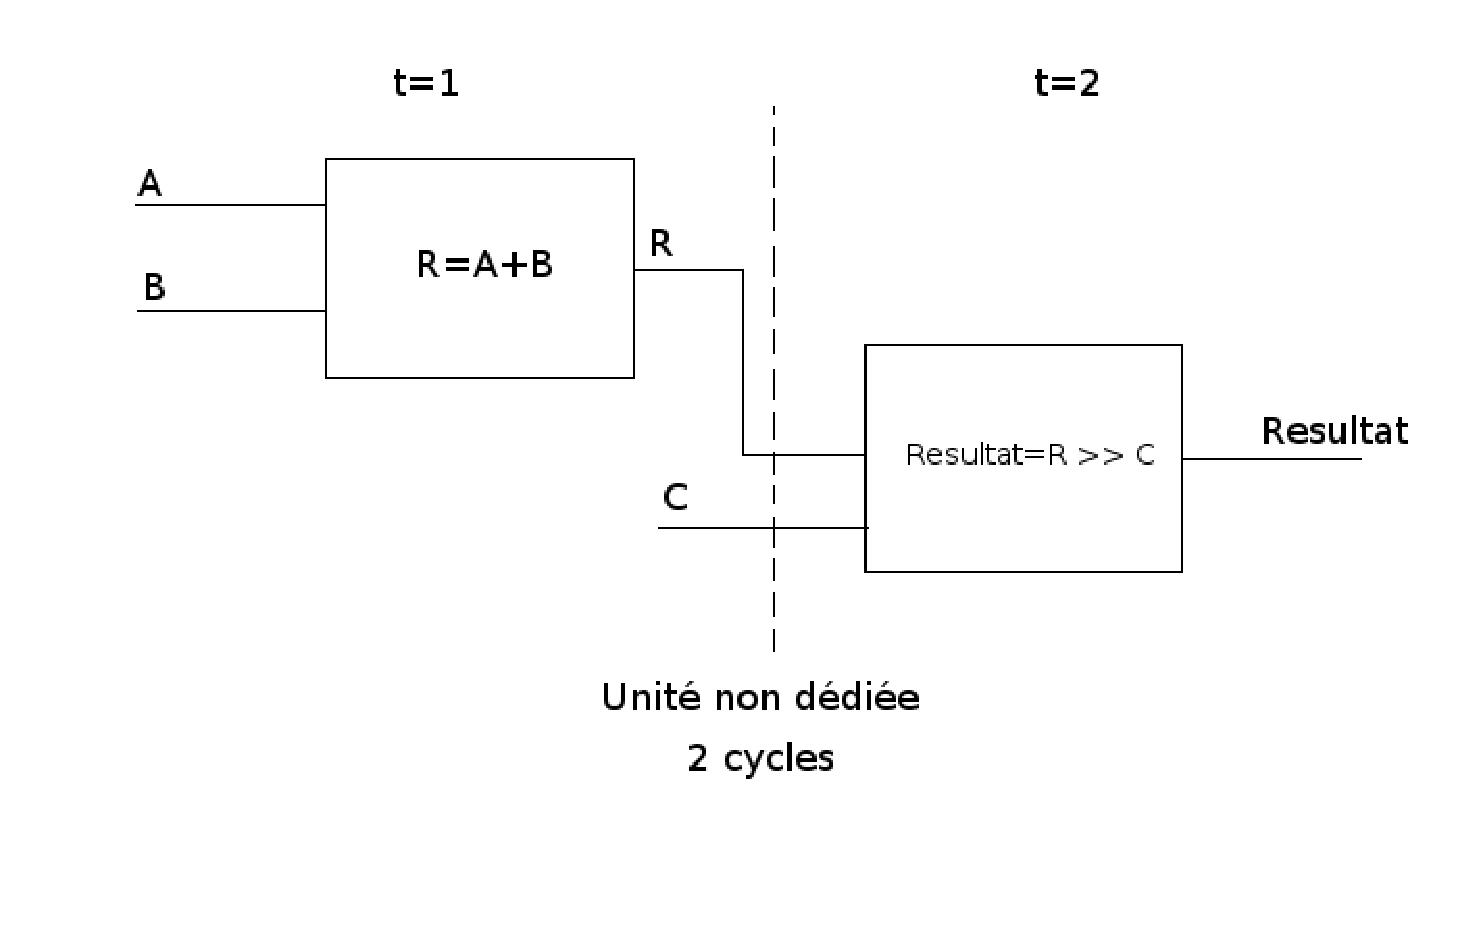
\includegraphics[scale=0.4]{bloc2.eps}
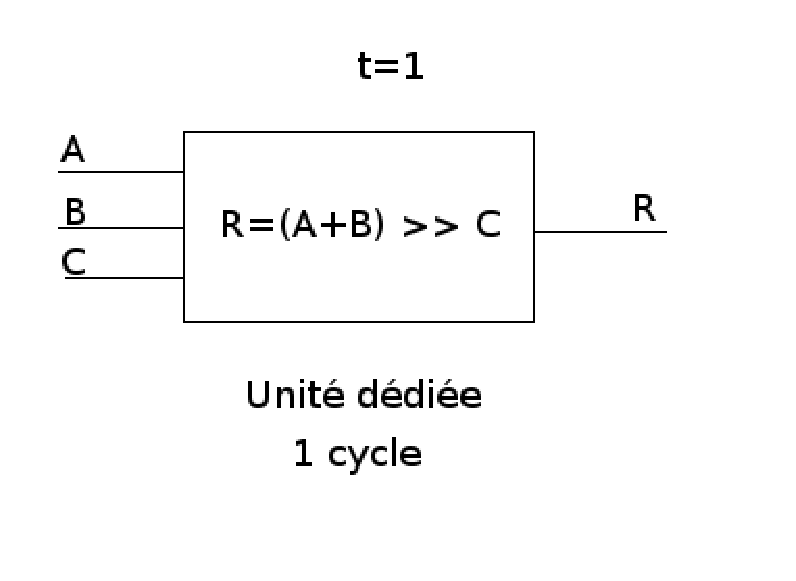
\includegraphics[scale=0.4]{bloc1.eps}
\end{center}
    \newpage

\chapter*{Conclusion}

\newpage
à faire

\end{document}

